\chapter{Proposed model}
\label{chap:model}
This section describes the proposed enhancements to the  +CityxChange \gls{eaf} to promote learning across cities in smart city development projects.
\section{Developed model} % or framework/tool/system add subsection by need

When developing the new model, as many issues as possible, from the original, should be solved. But there is a trade-off between complexity and coverage. Complexity should be low to encourage use by non-experts while coverage should be high to allow use in multiple situations and for correct usage. 

\subsection{Enhancements of the development process}
\begin{figure}
    \centering
    \makebox[\textwidth][c]{
        \rotatebox{-90}{
            %New development process
% Define block styles
\tikzset{
    decision/.style={diamond, draw, fill=blue!20, text centered, text width = 1.5cm},
    block/.style={rectangle, draw, fill=blue!20, rounded corners, text width = 1.8cm},
    mindset/.style={
        rectangle split, rectangle split parts=2, 
        rectangle split part fill={yellow!20,green!20},
        draw, text width=2.4cm},
    to/.style={draw, -latex},
    connect/.style={draw, dashed},
    textnode/.style={text width=0.5cm}
}

    
\begin{tikzpicture}[]
    % Main steps
    \node[block, left= 0.8cm of components] (users) {Consider users interested in this model};
    \node [block] (components) {Identify and describe components in horizontal layers};
    \node [block, right= 0.8cm of components] (documentation) {Identify documentation and knowledge reservoirs};
    \node[block, right= 0.8cm of documentation, yshift=1.2cm] (resources) {Identify and describe resources};
    \node [block, right= 0.8cm of documentation, yshift=-1.2cm] (relationships) {Identify and describe relationships};
    \node [block, right= 0.8cm of relationships, yshift=1.2cm] (perspectives) {Identify stakeholder and data perspectives};
    \node [decision, right= 0.5cm of perspectives] (iscomplete) {Is model complete};
    \node [block, above= 0.5cm of resources] (iterate) {Iterate to add detail};
    \node [block, right= 0.6cm of iscomplete] (views) {Identify views to visualise};

    % Mindset
    \node[mindset, below=0.8cm of users] (mindusers) { \nodepart{one} \begin{center} Mindset \end{center}
        \nodepart{two}
        \begin{itemize}[leftmargin=0.3cm]
            \item Why is the model needed?
            \item Who is the model for?
        \end{itemize}
    };
    
    \node[mindset, below=0.8cm of components] (mindcomponents) { \nodepart{one} \begin{center} Mindset \end{center}
        \nodepart{two}
        \begin{itemize}[leftmargin=0.3cm]
            \item What is relevant for the models users?
            \item What is needed to make decisions?
            \item How does the \gls{ea} look to outsiders?
        \end{itemize}
    };
    
    \node[mindset, below=0.8cm of documentation] (minddocumentation) { \nodepart{one} \begin{center} Mindset \end{center}
        \nodepart{two}
        \begin{itemize}[leftmargin=0.3cm]
            \item Where can users find more information?
            \item What documentation needs to be updated on changes?
        \end{itemize}
    };
    
    \node[mindset, below=0.8cm of relationships] (mindrelationships) { \nodepart{one}
    \begin{center} Mindset \end{center}
        \nodepart{two}
        \begin{itemize}[leftmargin=0.3cm]
            \item Who and what is communicated?
            \item Which protocols or processes do they use?
            \item Which techniques are used to share/retain knowledge?
            \item How is communication documented?
        \end{itemize}
    };
    
    \node[mindset, below=0.8cm of perspectives] (mindperspectives) { \nodepart{one}
    \begin{center} Mindset \end{center}
        \nodepart{two}
        \begin{itemize}[leftmargin=0.3cm]
            \item Who has an interest in the systems completion?
            \item Who participates in development?
        \end{itemize}
    };
    
    \node[mindset, below=0.8cm of views] (mindviews) { \nodepart{one}
    \begin{center} Mindset \end{center}
        \nodepart{two}
        \begin{itemize}[leftmargin=0.3cm]
            \item Do groups interpret the system differently?
            \item Do groups have different terminology?
            \item Are there things that are likely to be misinterpreted?
            \item Can unnecessary information be hidden?
        \end{itemize}
    };
    
    \node[mindset, below=1.5cm of iscomplete] (mindresources) { \nodepart{one}
    \begin{center} Mindset \end{center}
        \nodepart{two}
        \begin{itemize}[leftmargin=0.3cm]
            \item Have human resources been allocated?
            \item Have financial resources been allocated?
            \item Are there missing resources?
            \item Could resources improve the system?
        \end{itemize}
    };
    
    % Draw flow
    \path [to] (users.east) -- (components.west);
    \path [to] (components.east) -- (documentation.west);
    \path [to] (documentation.east) -| (4.3,-1.2) -- node [below, xshift=-0.2cm] {And} (relationships.west);
    \path [to] (documentation.east) -| (4.3,1.2) -- node [above, xshift=-0.2cm] {And} (resources.west);
    \path [to] (relationships.east) -| (7,0) -- (perspectives.west);
    \path [to] (resources.east) -| (7,0) -- (perspectives.west);
    \path [to] (perspectives.east) -- (iscomplete.west);
    \path [to] (iscomplete.north) |- node [right] {no} (iterate.east);
    \path [to] (iterate.west) -| (components.north);
    \path [to] (iscomplete.east) -- node [above] {yes} (views.west);
    
    % Draw supplimentary connections
    \path[connect] (users) -- (mindusers);
    \path[connect] (components) -- (mindcomponents);
    \path[connect] (documentation) -- (minddocumentation);
    \path[connect] (relationships) -- (mindrelationships);
    \path[connect] (perspectives) -- (mindperspectives);
    \path[connect] (views) -- (mindviews);
    \path[connect] (resources.north) |- (10, 2.5) |- (mindresources.north west);
\end{tikzpicture}


        }
    }
    \caption{Development process of an EA using the proposed model.}
    \label{fig:4-architecture-development-after}
\end{figure} %Collaboration layer
% Identify <Conspets>
% Component, entity Explain
% Explain mindset


The development process of an \gls{ea} has been altered, as shown in figure \ref{fig:4-architecture-development-after}, to allow for consideration of elements that are relevant to learning. It is meant as a guide and not meant to be used as a hard requirement. More specifically; three steps have been added.
\begin{itemize}
    \item \textbf{Consider users}: Added due to learning and \gls{ea} being concepts that are intrinsically linked to human efficiency and behaviour.
    \item \textbf{Knowledge identification}: Added as it is believed that the \gls{ea} model by itself will not be able to sufficiently cover everything each individual needs for learning, but can still guide the individual towards important information. It also forces the \gls{ea} architects to consider how knowledge is created within the system.
    \item \textbf{Resource identification}: Added due to resources being a concept that is repeatedly mentioned in the literature. Both when it comes to innovation and within smart city development due to the multi stakeholder context.
\end{itemize}

{\centering
\begin{longtable}{|p{6cm}|p{6cm}|}
    \hline
    Mindset & Relevant \gls{boundary object} properties \\ \hline
    Why is the model needed? & concreteness\\ \hline
    Who is the model for? & concreteness, malleability, participation \\ \hline

    What is relevant for the models users? & concreteness, malleability, participation\\ \hline
    What is needed to make decisions? & concreteness \\ \hline
    How does the \gls{ea} look to outsiders? & concreteness\\ \hline

    Where can users find more information? & concreteness, (indirect) accessibility \\ \hline
    What documentation needs to be updated on changes? &  Up-to-dateness \\ \hline

    Who and what is communicated? & concreteness \\ \hline
    Which protocols or processes do they use? & concreteness \\ \hline
    Which techniques are used to share/retain knowledge? & concreteness \\ \hline
    How is communication documented? & concreteness\\ \hline

    Who has an interest in the systems completion? & concreteness, malleability, participation \\ \hline
    Who participates in development? & concreteness, malleability, participation \\ \hline

    Do groups interpret the system differently? & shared syntax, annotation, modularity\\ \hline
    Do groups have different terminology? & shared syntax \\ \hline
    Are there things that are likely to be misinterpreted? & shared syntax \\ \hline
    Can unnecessary information be hidden? & modularity, visualization\\ \hline
    
    Have human resources been allocated? & concreteness \\ \hline
    Have financial resources been allocated? & concreteness, visualization \\ \hline
    Are there missing resources? & concreteness, visualization \\ \hline
    Could resources improve the system? & concreteness, visualization \\ \hline
    
    \caption{A mapping of the mindsets to relevant Boundary object properties}
    \label{tab:4-mindset-properties}
\end{longtable}}
Figure \ref{fig:4-architecture-development-after} also adds questions one can have in mind while developing the \gls{ea} model. The questions are called mindsets and are meant to make the intention behind the \gls{ea} model clearer to the architect and make them consider knowledge flows. A mindset in this context is a perspective or set of ideas that can influence decisions. This semi-structured approach is used as the concept of "learning" is hard to define or achieve in a rigid environment. The mindsets are a result of viewing the \gls{ea} model as a \gls{boundary object}, It does not use the specific terminology within the diagram, as it is not expected that the \gls{ea} architects are familiar with the concept. Table \ref{tab:4-mindset-properties} shows how the terminology applies to the mindsets. 

\subsection{Enhancements of the EAF}
\begin{figure}
    \centering
    %\begin{turn}{-90}
    \makebox[\textwidth][c]{
        \tikzset{
  box/.style={
    draw,
    rectangle,
    minimum height=1cm,
    fill=white,
    align=center,
    inner sep=1ex
  }
}

\begin{tikzpicture}[]
    \iffalse
    \begin{scope}[on background layer]
         \node at (-0.5,-3) [box, minimum width=2.5cm, text width=1.8cm, minimum height=9cm, fill=cyan, align=north] (planning) {Integrated Planning and design};
        \node[box, minimum width=2.5cm, text width=1.8cm, minimum height=9cm, fill=cyan, right= 2mm of planning] (common) {Common energy market};
        \node[box, minimum width=2.5cm, text width=1.8cm, minimum height=9cm, fill=cyan, right= 2mm of common] (community) {Community- xChange};   
    \end{scope}
    \fi
    %Horizontal - Inner
    \node[box, opacity=0.8, text width=\textwidth/2]  (process) {processes and internal initiatives};
    \node[box, opacity=0.8, text width=\textwidth/2, below=2mm of process]  (team) {Team structures};
    \node[box, opacity=0.8, below=2mm of team, text width=\textwidth/1.8]  (goal) {Goals and KPIs};
    \node[box, opacity=0.8, below=2mm of goal, text width=\textwidth/2] (service) {Value Added Services};
    \node[box, opacity=0.8, below=2mm of service, text width=\textwidth/2]  (business) {Enterprise cooperation};
    \node[box, opacity=0.8, below=2mm of business, text width=\textwidth/2]  (application) {Application and Data Processing};
    \node[box, opacity=0.8, below=2mm of application, text width=\textwidth/2]  (data) {Data Space};
    \node[box, opacity=0.8, below=2mm of data, text width=\textwidth/2]  (technology) {Technologies};
    \node[box, opacity=0.8, below=2mm of technology, text width=\textwidth/2]  (physical) {Physical Infrastructure};

    % Context - Outer
    \begin{scope}[on background layer]
        \node[box, opacity=0.1, inner sep=1ex, fit=(process) (team) (goal) (service) (business) (application) (data) (technology) (physical)] (main) {};
    \end{scope}

    % Stakeholder perspective  - Inner
    \node[box, minimum height=\textwidth/2, left=of main] (ownership) {\rotatebox{90}{Ownership and access}};
    \node[box, minimum height=\textwidth/2, left=2mm of ownership] (privacy) {\rotatebox{90}{Privacy \& Trust}};
    \node[box, minimum height=\textwidth/2, left=2mm of privacy] (policy) {\rotatebox{90}{Policies \& Regulations}};
    \node[box, minimum height=\textwidth/2, left=2mm of policy] (stakeholder) {\rotatebox{90}{Stakeholders}};

    % Stakeholder perspective  - Outer
    \begin{scope}[on background layer]
        \node[box, inner sep=1ex, fit=(stakeholder) (policy) (privacy) (ownership),  label={Stakeholder perspective}] (stakeholder) {};
    \end{scope} 

    % Data perspective - Inner    
    \node[box, minimum height=\textwidth/2, right=of main] (interoperability) {\rotatebox{90}{interoperability}};
    \node[box, minimum height=\textwidth/2, right=2mm of interoperability] (security) {\rotatebox{90}{Data security, Risk assessment}};
    \node[box, minimum height=\textwidth/2, right=2mm of security] (governance) {\rotatebox{90}{Data Governance}};
    
    % Stakeholder perspective  - Outer
    \begin{scope}[on background layer]
        \node[box, inner sep=1ex, fit=(interoperability) (security) (governance),  label={Data perspective}] (stakeholder) {};
    \end{scope} 

\end{tikzpicture}
    }%
    %\end{turn}
    \caption{Proposed EAF based on the +CityxChange EAF}
    \label{fig:4-architecture-after}
\end{figure}


As shown in figure \ref{fig:4-architecture-after} and \ref{fig:4-architecture-elements} the \gls{eaf} has been expanded and more architectural elements have been added. Although this could intuitively increase complexity, the intent is that a further segmentation of the domain and greater specificity with better concreteness, shared syntax and visualization, can make the model more intuitive and allow more relevant views for individuals. 

The original context layer has been expanded to three layers; "goals and \glspl{kpi}", "Team structures" and "processes and internal initiatives". The "goals and \glspl{kpi}" layer is intended to be used like the context layer was used in the original. It contains the core motivations behind the system(s) being developing. Figure \ref{fig:4-architecture-after} shows this layer being accentuated. This is because it is considered to be vital for decision making. "Team structures" and "Processes and internal initiatives" were placed above, not because of higher significance, but because they are further removed from the application and physical infrastructure layers. The added "Team structures" layer is for documenting internal teams working on development. It is intended to help understand how knowledge flows between people and groups. It is different from the layer in the origin \gls{eaf} called "Business (Virtual Enterprise)" and called "Enterprise collaboration" in the proposed \gls{eaf} in that the collaboration layer contains companies or stakeholders involved in the development rather than internal structures that might be specific to each stakeholder. "Processes and internal initiatives" is the final layer that has been changed from the original. It is meant to capture more of the knowledge flows by adding processes that are initiated and heavily governed by peoples, such as daily meetings and workshops. 

\subsection{Addition EA elements}
\begin{figure}
    \centering
    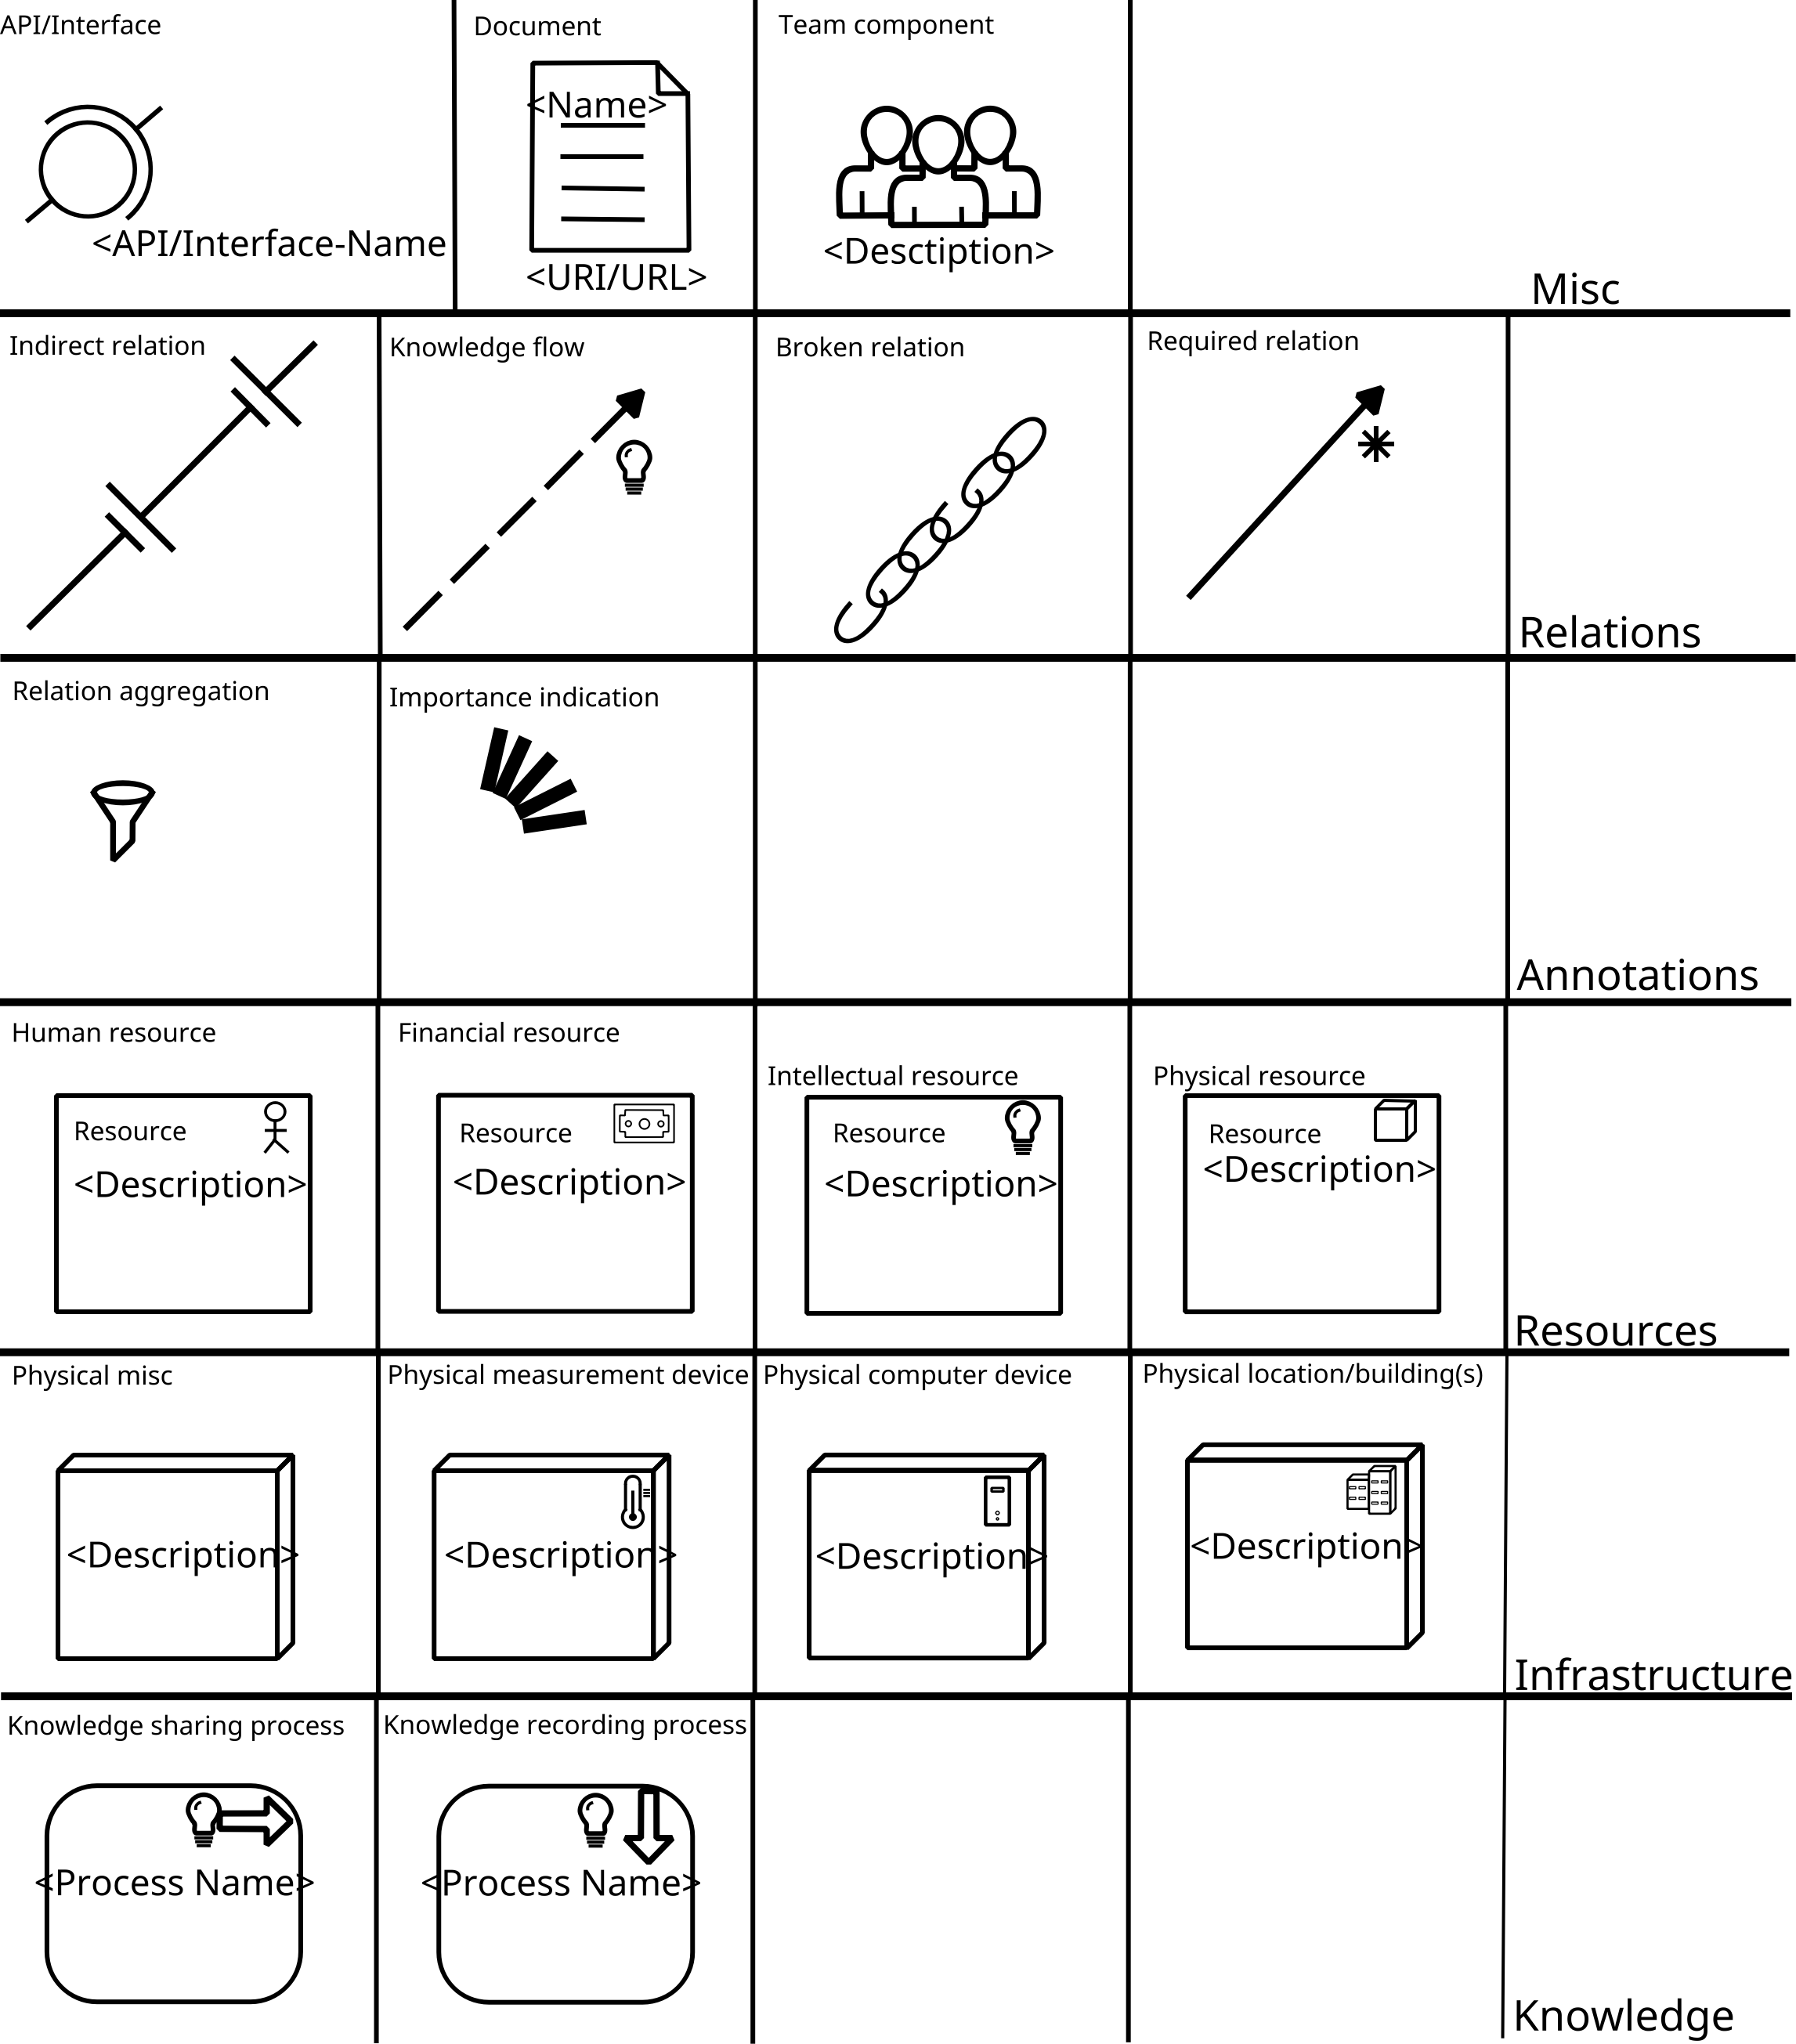
\includegraphics[scale=0.6]{figures/png/elements.png}
    \caption{Proposed elements for making EA models from proposed EAF }
    \label{fig:4-architecture-elements}
\end{figure}

Figure \ref{fig:4-architecture-elements} shows the proposed elements that can be used to create the \gls{ea} models. It is meant to supplement or enhance the elements in \gls{togaf}. \gls{togaf} was used as a base due to its current use within +CityxChange and recommendation by multiple relevant articles \cite{7580810, pourzolfaghar2016types}.
Some of the elements, such as aggregation and indirect connections, have been added to allow views to partially be created logically from a base \gls{ea} model allowing further hiding of irrelevant information. while other elements are meant to include knowledge related components or better represent the smart city context.

\begin{itemize}
    \item \textbf{Api/interface} element is an alteration of the \gls{togaf} interface elements. It has been changed so that it is more clearly differentiated from the other elements. This was done as the \glspl{api} were a topic mentioned repeatedly in +CityxChange meetings and are seen as important parts of the \gls{ea}.
    \item \textbf{Document} element is a  more general version of \gls{togaf} artefact that also has a \gls{url}/\gls{uri}. This \gls{url}/\gls{uri} was added to improve the accessibility of the document.\Gls{the open group} defines an artefact as "a physical piece of data that is used or produced in a software development process, or by deployment and operation of a system."\cite{archilayer}. The proposed document is not tied to the software, but can be things like meeting notes.
    \item \textbf{Team component} was added because humans are the core of any knowledge related activity.
    \item \textbf{Indirect relation} was added to allow hiding of connected elements in certain views without hiding the connections between the other elements.
    \item \textbf{Knowledge flow} shows how knowledge flows in the \gls{ea} and was added to make knowledge information more specific.
    \item \textbf{Broken relation} shows that a connection is expected or preferred, but not implemented. This was added to visualise potential areas for improvement or innovation.
    \item \textbf{Required relation} shows that a connection can not be removed without significant work. This was added to allow separate communities to give additional information about what is necessary from their perspective.
    \item \textbf{Relation aggregation} was added as the multi stakeholder context often require many to one connections and a way to remove clutter could improve visualisation. It might also be beneficial for views where components with several connections are hidden. 
    \item \textbf{Importance indicator} is meant to attach to other components to indicate that the user of the \gls{ea} model might want to consider that component. It can be relevant to add this to specific views as importance is dependent on perspective.
    \item \textbf{Resources} elements expand the \gls{togaf} resource element with four more specific version and a new notation. The versions are human financial, intellectual and physical resources respectively. These were added based on their importance for innovation capabilities.
    \item \textbf{Physical entities} were added as the smart city concept often revolve around physical infrastructure such as chargers for \gls{emaas}, sensors for data gathering and smart grids. The \gls{togaf} node element is changed into a physical misc element for generic physical components and specific elements were added for measurement, computation devices and locations.
    \item \textbf{Knowledge processes} were added to show how the knowledge flows within the \gls{ea}, how it is shared and how it is recorded.
\end{itemize}
 
Some of the unchanged elements from \gls{togaf} that are seen as important are; the influence relation, the stakeholder and goals/\gls{kpi} related elements, principle element and note. 
{\centering
\begin{longtable}{|p{2.3cm}|p{4.5cm}|p{5cm}|}
    \hline
        Grouping & Element & Description/attribute\\ \hline
        \multirow{3}*{Misc} 
            & \multirow{4}*{API or interface} & Used to indicate \gls{api} or interfaces. \\ \cline{3-3}
            & & Attribute: \gls{api} name. \\ \cline{3-3}
            & & Attribute: \gls{api} ID for lookup. \\ \cline{3-3}
            & & Attribute: File link or \gls{uri}. \\ \cline{2-3}
            & \multirow{7}*{Document} & Used to represent documentation or artefact stored outside the current \gls{ea} model. \\ \cline{3-3}
            & & Can be used refer to other \gls{ea} components, \gls{uml} diagram, organisational charts, system specifications, resource allocations, etc. \\ \cline{3-3}
            & & Attribute: File name. \\ \cline{3-3}
            & & Attribute: File description. \\ \cline{3-3}
            & & Attribute: File link or \gls{uri}. \\ \cline{3-3}
            & & Attribute: File access description (if link or \gls{uri} is not applicable). \\ \cline{3-3}
            & & Attribute: File type or comprehension. \\ \cline{2-3}
            & \multirow{1}*{Organisational component} &  Used to represent a team, group or other organisational structure. \\
        \hline
        \multirow{4}*{Relations} 
            & \multirow{1}*{Indirect relation} &  Used to show an indirect relationship that should be known. \\  \cline{2-3}
            & \multirow{1}*{Knowledge flow} & Used to show how knowledge flows or is created. \\ \cline{2-3}
            & \multirow{1}*{Broken relation} & Used to show that a relation is expected, but not implemented or functional. \\ \cline{2-3}
            & \multirow{1}*{Required relation} & Used to show that a relationship can not be removed. \\
        \hline
        \multirow{2}*{Annotation}
            & \multirow{1}*{Relation aggregation} &  Used to simplify visualisation of many to one or many to many relationships. \\ \cline{2-3}
            & \multirow{2}*{Importance indicator} &  Used to show that a component or relation is important for development or decision making. \\ \cline{3-3}
            & & Attribute: Justification \\
        \hline
        \multirow{4}*{Resources}
            & \multirow{5}*{Resource misc} & Used to represent a resource, when no other element can be more descriptive. \\ \cline{3-3}
            & & Attribute: Resource type. \\ \cline{3-3}
            & & Attribute: Resource quantity. \\ \cline{3-3}
            & & Attribute: Resource description. \\ \cline{3-3}
            & & Attribute: Resource justification.\\ \cline{2-3}
            & \multirow{4}*{Human Resource} & Used to represent a human resource. \\ \cline{3-3}
            & & Attribute: Resource quantity. \\ \cline{3-3}
            & & Attribute: Resource description. \\ \cline{3-3}
            & & Attribute: Resource justification.\\ \cline{2-3}
            & \multirow{4}*{Intellectual Resource} & Used to represent a knowledge based resource. \\ \cline{3-3}
            & & Attribute: Resource quantity. \\ \cline{3-3}
            & & Attribute: Resource description. \\ \cline{3-3}
            & & Attribute: Resource justification.\\ \cline{2-3}
            & \multirow{4}*{Physical Resource} & Used to represent a resource with physical properties. \\ \cline{3-3}
            & & Attribute: Resource quantity. \\ \cline{3-3}
            & & Attribute: Resource description. \\ \cline{3-3}
            & & Attribute: Resource justification.\\ \cline{2-3}
        \multirow{4}*{Infrastructure} 
            & \multirow{1}*{Physical misc} & Used to represent a physical entity when no other element is more descriptive. \\ \cline{3-3}
            & & Attribute: Type. \\ \cline{3-3}
            & & Attribute: Description. \\ \cline{2-3}
            & \multirow{1}*{Physical measurement device} & Used to represent data-gathering devices. \\ \cline{3-3}
            & & Attribute: Data type. \\ \cline{3-3}
            & & Attribute: Description. \\ \cline{2-3}
            & \multirow{1}*{Physical computation device} & Used to represent computing devices, servers or similar. \\ \cline{3-3}
            & & Attribute: Capability. \\ \cline{3-3}
            & & Attribute: Description. \\ \cline{2-3}
            & \multirow{1}*{Physical location/building} & Used to represent important locations or buildings. \\ 
        \hline
        \multirow{2}*{Knowledge} 
            & \multirow{1}*{Knowledge sharing process} & Used to represent activities such as meetings, workshops etc that share knowledge between individuals or groups. \\ \cline{3-3}
            & & Attribute: Process name. \\ \cline{3-3}
            & & Attribute: Knowledge description. \\ \cline{2-3}
            & \multirow{1}*{Knowledge recording process} & Used to represent activities such as document writing, meeting recording etc that result in tacit knowledge being converted to explicit knowledge. \\ \cline{3-3}
            & & Attribute: Process name. \\ \cline{3-3}
            & & Attribute: Knowledge description. \\
    \hline
    
    \caption{Suggested elements represented in the EA model and optional attributes of those.}
    \label{tab:4-element-attributes}
\end{longtable}}

Table \ref{tab:4-element-attributes} shows a more detailed view of the suggested elements. It adds attributes on some elements that might not be visible on the component, but can be added in a digital representation and viewed when a component is selected.  

\section{Summary}
This chapter presented an enhanced \gls{eaf} along with a \gls{ea} development process and \gls{ea} elements that can be used to represent an \gls{ea} that could support the transfer of learning across cities. The model builds on the +CityxChange \gls{eaf} and \gls{togaf}, and is intended to promote learning in a smart city context.